\begin{boiboiboite}
	\propair
	\propgaz
	\isentropiques
\end{boiboiboite}

\subsubsection{Quelques questions de cours}

	\begin{itemize}
		\item Représentez le cycle suivi par l’air dans un turboréacteur simple flux monoturbine sur un diagramme pression-volume et température-entropie.
		\item Pourquoi utilise-t-on deux arbres moteur concentriques (et donc deux ensembles compresseur+turbine) dans certaines turbomachines ?
		\item Représentez le cycle suivi par l’air dans un turbomoteur à refroidisseur intermédiaire et échangeur économiseur (\cref{fig_intercooler_echangeur}) sur un diagramme température-entropie.
	\end{itemize}


\subsubsection{Générateur à refroidissement intermédiaire}

	Une installation portative légère est conçue pour générer de l’électricité de façon autonome. Elle comporte un seul axe (compresseur et turbine uniques) et a les propriétés suivantes :
	\begin{itemize}
		\item Rapport de pressions $\frac{p_\text{max.}}{p_\text{min.}}$ :  	\tab \num{10}
		\item Efficacité compresseur :  									\tab \SI{78}{\percent}
		\item Température d’entrée turbine : 							\tab \SI{1200}{\kelvin}
		\item Efficacité turbine : 										\tab \SI{88}{\percent}
		\item Efficacité mécanique de l’axe : 							\tab \SI{95}{\percent}
		\item Entrée compresseur : 										\tab \SI{295}{\kelvin} et~\SI{1,015}{\bar}
	\end{itemize}

	\begin{enumerate}
		\item Schématisez le circuit suivi par l’air dans le moteur, et tracez le cycle thermodynamique sur un diagramme température-entropie.
		\item Quelle est la puissance mécanique développée par l’installation ?
		\item Quels sont son rendement et son rapport des puissances ?
	\end{enumerate}
	
	On décide d’améliorer le moteur en séparant la compression en deux étapes, et en insérant un refroidisseur (intercooler) entre ces deux étapes.\\
	Désormais, la compression est interrompue à~\SI{3,21}{\bar}, et l’air est alors refroidi à pression constante jusqu’à~\SI{370}{\kelvin}.\\
	La compression est ensuite poursuivie et le même rapport de pressions global $\frac{p_\text{max.}}{p_\text{min.}}$ est obtenu.
	
	\begin{enumerate}
		\shift{3}
		\item Schématisez le nouveau circuit suivi par l’air et le diagramme température-entropie correspondant.
		\item Quelle est la nouvelle puissance fournie ?
		\item Quelles sont les nouvelles valeurs du rendement et du rapport des puissances ?
	\end{enumerate}

\subsubsection{Turbopropulseur}

	\wherefrom{[calqué sur partiel 2010, 7pts]}
	
	Un avion de ligne régional est motorisé par deux turbopropulseurs (\cref{fig_turboprop_photos}). Dans chacun d’entre eux, une turbine unique alimente un compresseur axial, ainsi que l’hélice par l’intermédiaire d’un réducteur (\cref{fig_turboprop_circuit}).
	
	\begin{figure}
		\begin{center}
			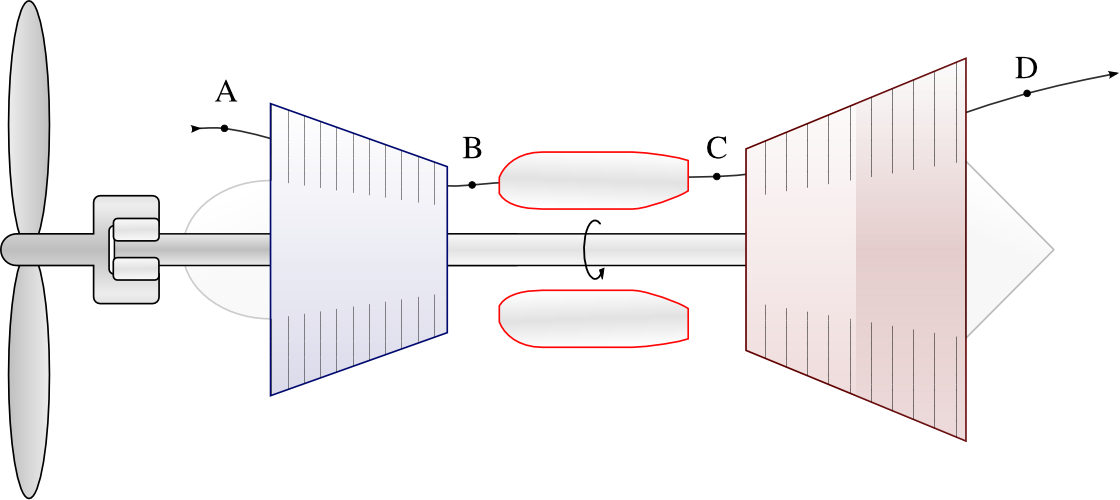
\includegraphics[width=11cm]{images/circuit_turboprop.png}
		\end{center}
		\supercaption{Circuit de principe d’un turbopropulseur.}{\ccbysa \olivier}
		\label{fig_turboprop_circuit}
	\end{figure}
	
	Pendant la croisière, le débit d’air au sein du moteur est de~\SI{4,9}{\kilogram\per\second}, et le circuit est le suivant :
	\begin{itemize}
		\item L’air à pression et température ambiantes (\SI{0,8}{\bar}, \SI{-5}{\degreeCelsius}) est admis dans le compresseur ;
		\item Le compresseur porte l’air à pression de~\SI{7,6}{\bar} avec une efficacité isentropique de~\SI{80}{\percent} ;
		\item L’air est ensuite chauffé dans la chambre de combustion jusqu’à~\SI{1070}{\degreeCelsius} ;
		\item Les gaz de combustion sont ensuite détendus dans la turbine et rejetés dans l’atmosphère ; La turbine a une efficacité isentropique de~\SI{80}{\percent}.
	\end{itemize}
	
	 La turbine alimente le compresseur (par l’intermédiaire d’un axe aux frottements négligeables), et l’hélice (par l’intermédiaire d’une boîte de transmission de rendement~\SI{92}{\percent}).
	
	Nous souhaitons quantifier la puissance effectivement reçue par l’hélice au cours du vol.
	
	\begin{enumerate}
		\item Tracez le cycle suivi par l’air sur un diagramme température-entropie.
		\item Quelle est la température à la sortie du compresseur ?
		\item Quelle est la température à la sortie de la turbine ?
		\item Quelle est la puissance reçue par l’hélice ?
	\end{enumerate}

	Afin de procéder au dégivrage des ailes, on propose d’effectuer un petit prélèvement de gaz au sein du compresseur. Le débit du prélèvement est de~\SI{0,1}{\kilogram\per\second}, et la température de l’air est de~\SI{200}{\degreeCelsius}.
	
	\begin{enumerate}
		\shift{4}
		\item Proposez et quantifiez une modification au cycle pour pouvoir maintenir la même puissance à l’hélice.
	\end{enumerate}
	
	\begin{figure}
		\begin{center}
			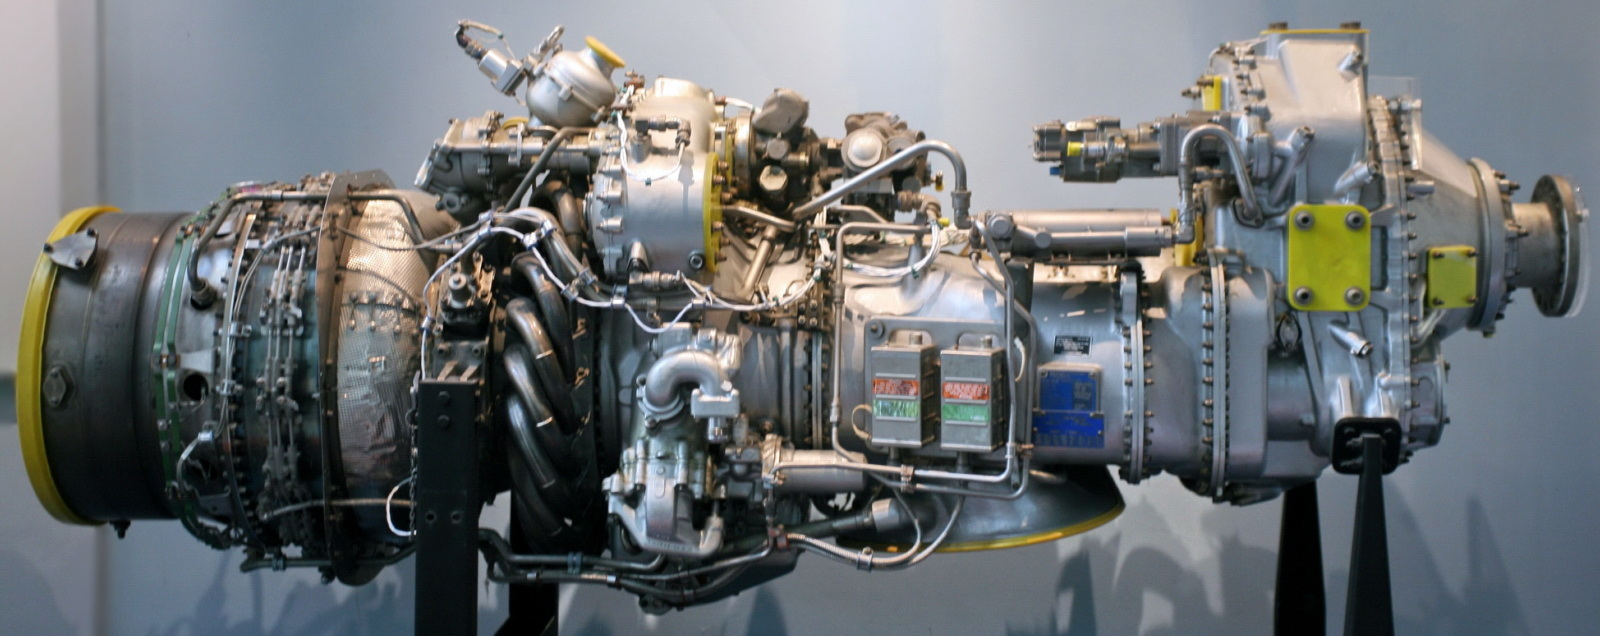
\includegraphics[height=0.245\textwidth]{images/photo_pwc_pw123.jpg}
			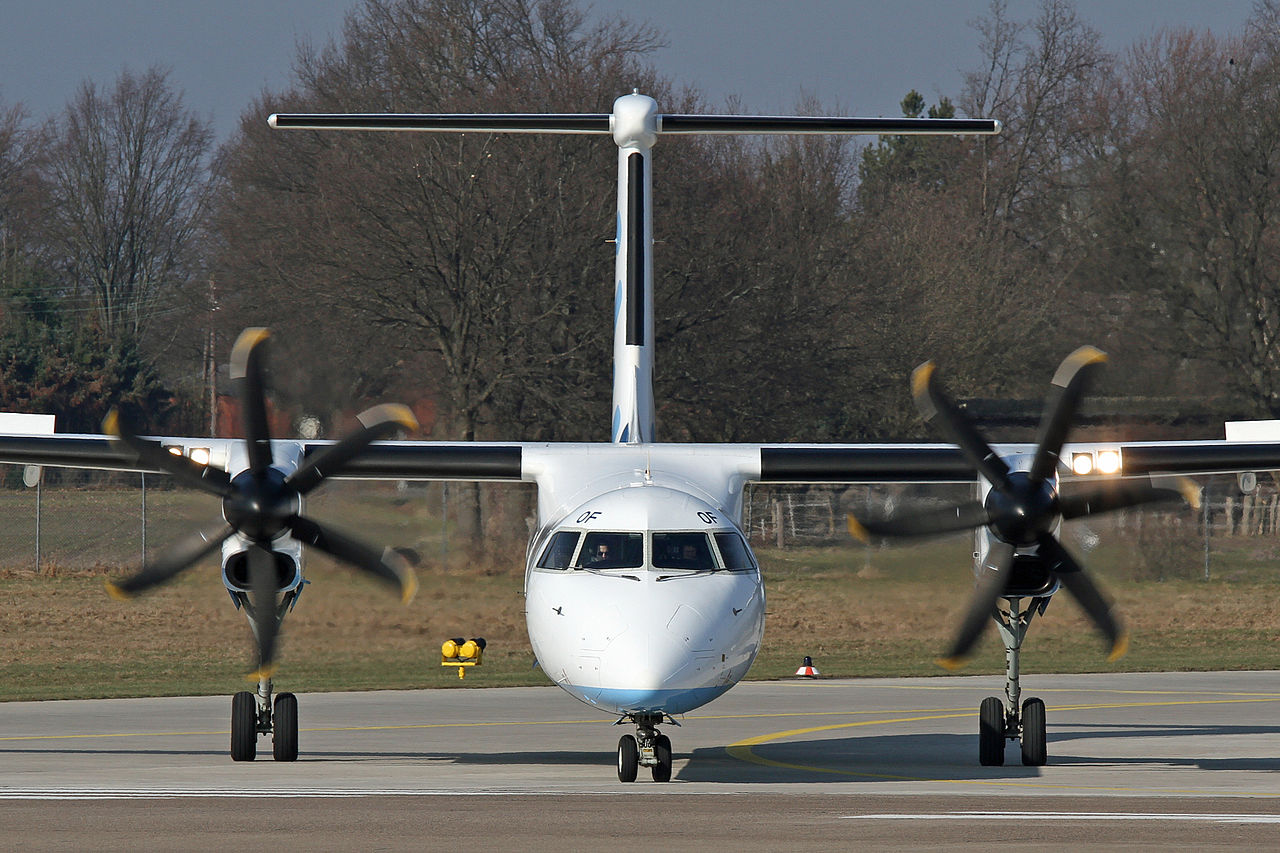
\includegraphics[height=0.245\textwidth]{images/photo_dash8.jpg}
		\end{center}
		\supercaption{Un turbopropulseur \textit{Pratt \& Whitney Canada} PWC123 équipant un Bombardier Dash~8. Le PWC123 est équipé de deux arbres et d’une turbine libre, mais son agencement de principe reste similaire à celui décrit en \cref{fig_turboprop_circuit}.}{Photo moteur dérivée d’\wcfile{Pratt_\%26_Whitney_Canada_PW123.jpg}{une photo} \ccby par \href{http://www.flickr.com/people/28567825@N03}{l’utilisateur/rice flickr cliff1066} ;\\ \wcfile{Dash_8_front_view.jpg}{Photo Dash 8} \ccbysa par \href{http://www.flickr.com/people/24056116@N07}{l’utilisateur/rice Flickr Björn}}
		\label{fig_turboprop_photos}
	\end{figure}
		

\subsubsection{Modification de turboréacteur}

	Un turboréacteur fonctionne avec un seul axe moteur (compresseur unique, et turbine unique). Ses caractéristiques de fonctionnement sont les suivantes :
		\begin{itemize}
			\item Débit d’air :							\tab \SI{4}{\kilogram\per\second} ; 
			\item Conditions atmosphériques : 		\tab \SI{10}{\degreeCelsius} et~\SI{0,95}{\bar}
			\item Rapport de pression $\frac{p_\text{max.}}{p_\text{min.}}$ : 				\tab \num{25}
			\item Température maximale : 													\tab \SI{1300}{\kelvin}
			\item Efficacité isentropique du compresseur et de la turbine : 	\SI{85}{\percent}
		\end{itemize}
	
	On cherche à quantifier ses performances avant modification.
		\begin{enumerate}
			\item Représentez les composants du turboréacteur, et le cycle thermodynamique suivi par l’air sur un diagramme température-entropie ou pression-volume.
			\item Quelle est la pression disponible à la sortie de la turbine ?
			\item Quelle serait la vitesse atteinte par les gaz en sortie de tuyère si la détente y était isentropique ?
		\end{enumerate}
		
		L’équipe d’ingénieurs en charge de la conception des composants propose de modifier le moteur, en utilisant deux axes plutôt qu’un seul (\cref{fig_exo_turbojet_twin_spool}). L’axe au centre de la turbine pouvant tourner à plus grande vitesse, l’efficacité isentropique des composants est augmentée :
			\begin{itemize}
				\item Efficacité isentropique du compresseur et de la turbine basse pression (axe BP) : \SI{85}{\percent}\\
					(rapport des pressions : \num{2})
				\item Efficacité isentropique du compresseur et de la turbine haute pression (axe HP) : \SI{90}{\percent}\\
					(rapport des pressions : \num{12,5})
			\end{itemize}
	
	\begin{figure}
		\begin{center}
			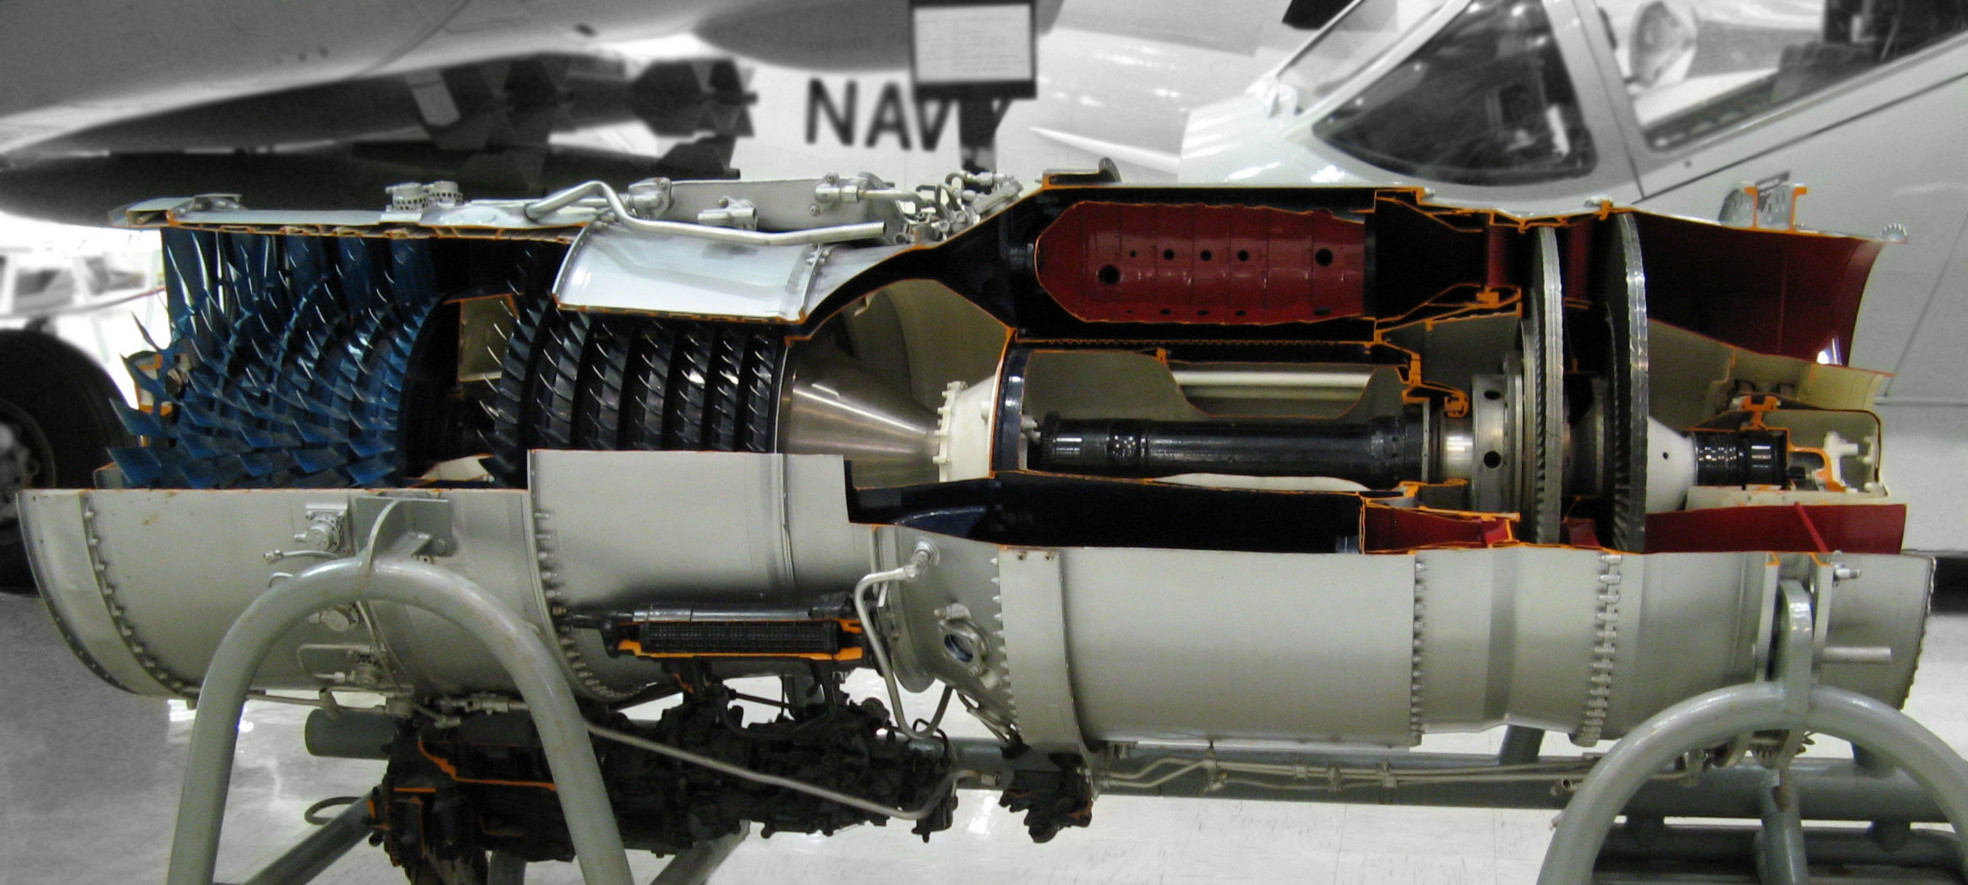
\includegraphics[height=0.27\textwidth]{images/photo_pw_j52_1.jpg}
			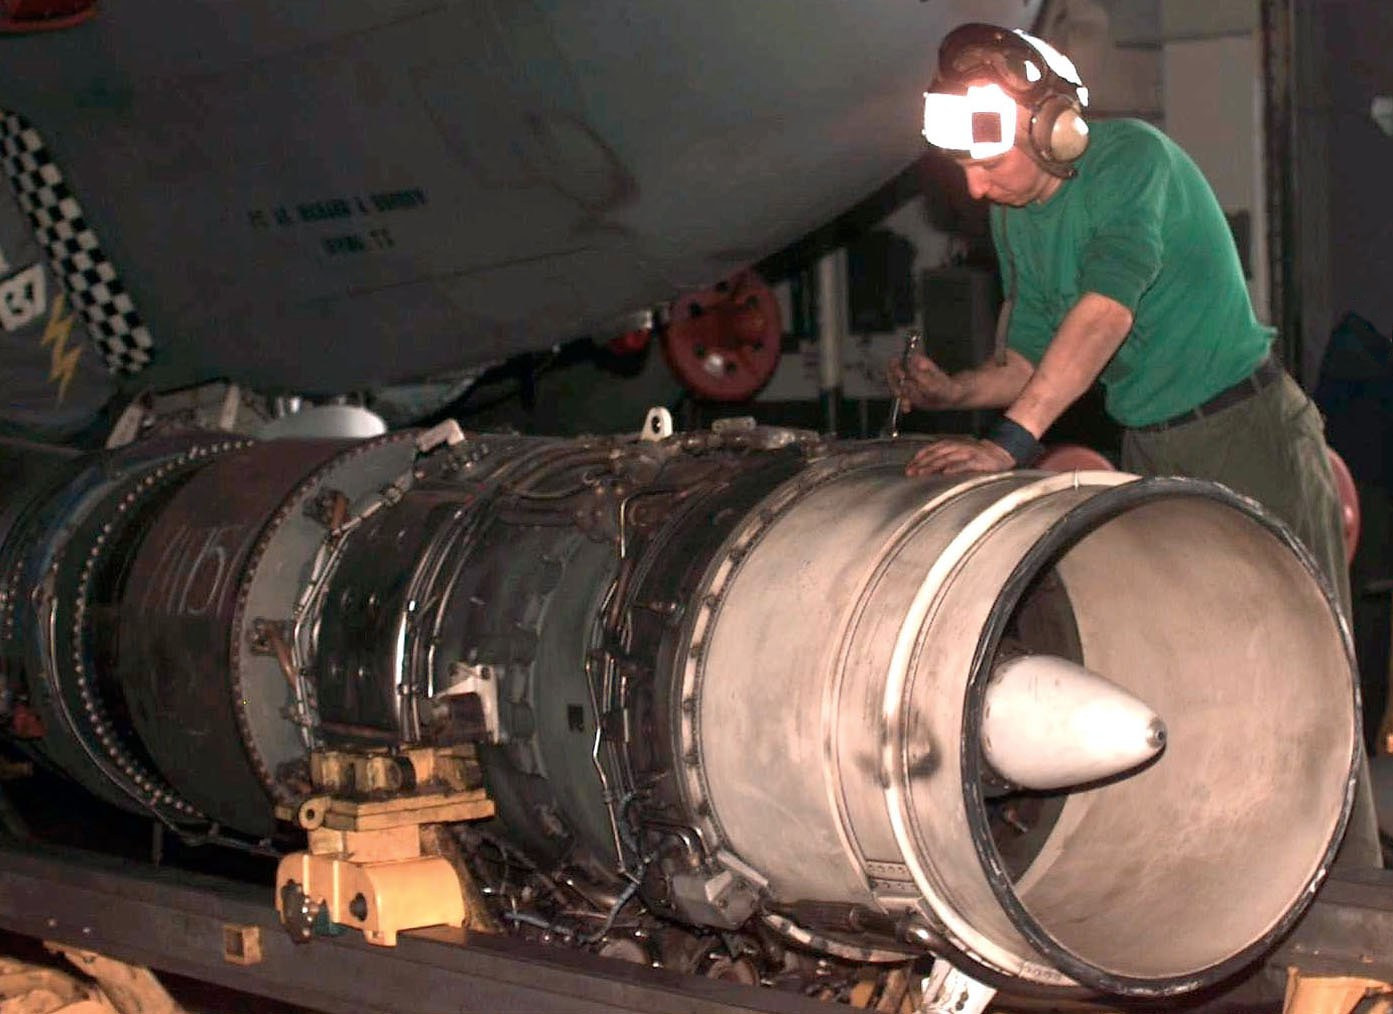
\includegraphics[height=0.27\textwidth]{images/photo_pw_j52_2.jpg}
		\end{center}
		\supercaption{Un turboréacteur à simple flux et deux arbres \wed{Pratt & Whitney J52}{\textit{Pratt \& Whitney} J52} (ou JT8A), construit en 4500 exemplaires. Il équipe encore le \wed{Northrop Grumman EA-6B Prowler}{EA-6B \textit{Prowler}}.}{Photo gauche dérivée d’\wcfile{Pratt_\%26_Whitney_J52.jpg}{une photo} \ccby par \href{http://www.flickr.com/people/37467370@N08}{Greg Goebel} ;\\ Photo droite dérivée d’\wcfile{J52_engine_maintenance_USS_America_(CV-66)_1993.JPEG}{une photo} \pd par Sgt.G. Robinson, U.S. Navy}
		\label{fig_exo_turbojet_twin_spool}
	\end{figure}
			
		Toutes les autres caractéristiques de fonctionnement du moteur restent inchangées.
		
		\begin{enumerate}
		\shift{3}
			\item Quelle est la nouvelle pression disponible à la sortie de la turbine ?
			\item Quelle est la nouvelle vitesse d’éjection des gaz ?
		\end{enumerate}


\subsubsection{Moteur à essence}

	\wherefrom{[partiel 2011, 6,5pts]}

	Nous nous proposons d’étudier le cycle théorique du moteur à pistons/cylindres d’un avion de tourisme (\cref{fig_photos_moteur_essence}). Le moteur est dit «~à essence~» et est basé sur le cycle théorique d’Otto.
La compression et la détente sont isentropiques ; l’apport et le rejet de chaleur se font à volume constant.
	
	\begin{figure}
		\begin{center}
			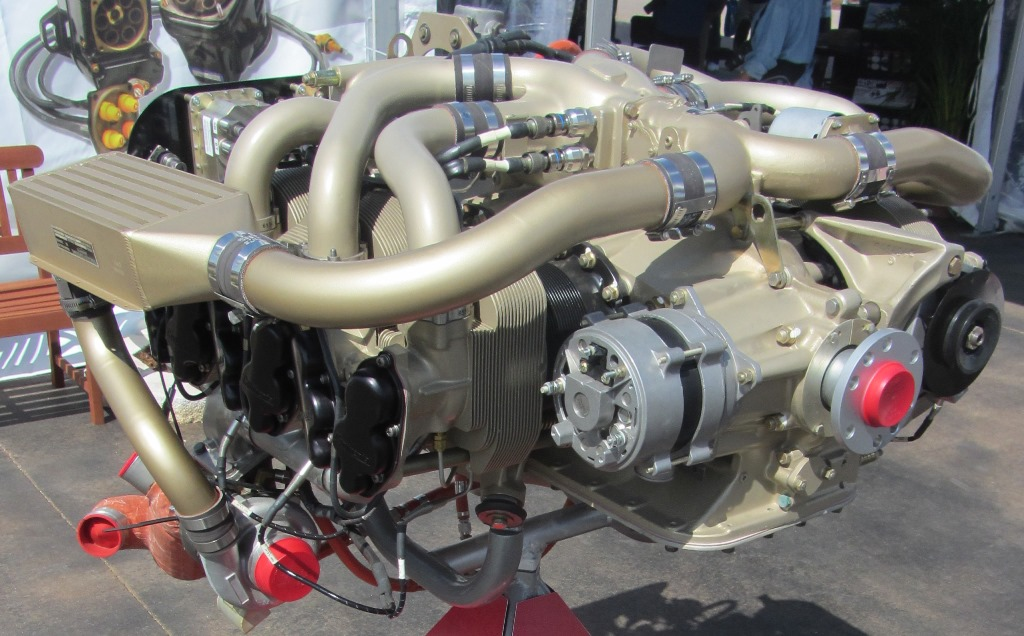
\includegraphics[height=0.315\textwidth]{images/photo_continental_io-550.jpg}
			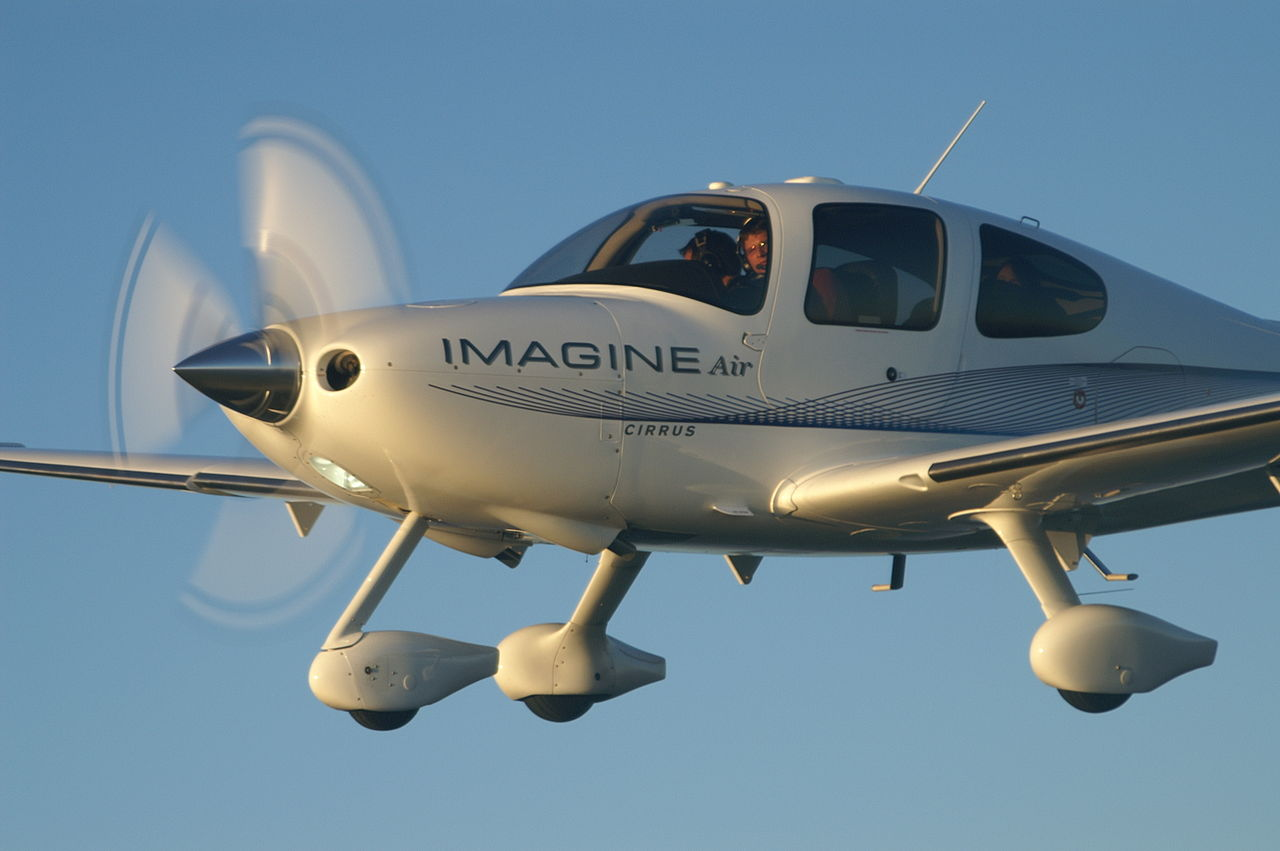
\includegraphics[height=0.315\textwidth]{images/photo_sr22.jpg}
		\end{center}
		\supercaption{Moteur six cylindres essence injection \we{Continental IO-550} de~\SI{300}{ch}, en fabrication depuis 1983. Il équipe entre autres le \we{Cirrus SR22}.}{\wcfile{TSIOF-550-D.jpg}{Photo gauche} \ccbysa par \wcu{FlugKerl2} ;\\ \wcfile{IAcirrus.JPG}{Photo droite} \ccbysa par \wcu{Airman7474}.}
		\label{fig_photos_moteur_essence}
	\end{figure}
	
	\begin{itemize}
		\item Au début du cycle, l’air est à~\SI{21}{\degreeCelsius} et~\SI{1}{\bar} ; 
		\item La chaleur spécifique fournie chaque cycle est de~\SI{500}{\kilo\joule\per\kilogram} ;
		\item Le taux de compression $\frac{V_\text{max.}}{V_\text{min.}}$ est de~\num{7}.
	\end{itemize}

	\begin{enumerate}
		\item Tracez le cycle suivi sur un diagramme pression-volume ou température-entropie, en y indiquant tous les transferts de chaleur et de travail.
		\item Quelles sont les températures de l’air au début et à la fin de la combustion ?
		\item Quelle est la quantité de chaleur rejetée lors du refroidissement ?
		\item Quel est le rendement de ce cycle théorique ?
		\item En pratique, l’évolution de l’air sur le diagramme pression-volume est fort différente du cycle décrit par Otto. Proposez deux raisons expliquant cela.
		\item On constate que lorsque l’appareil gagne de l’altitude, la puissance que le moteur peut fournir baisse très significativement. Quelle modification peut-on apporter au moteur pour compenser cela ?
	\end{enumerate}


\subsubsection{Moteur Diesel}

	\wherefrom{[partiel 2010, 8pts]}

	Un moteur à pistons-cylindres fonctionne sur le cycle théorique de Diesel, avec les caractéristiques suivantes :
	
	\begin{figure}
		\begin{center}
			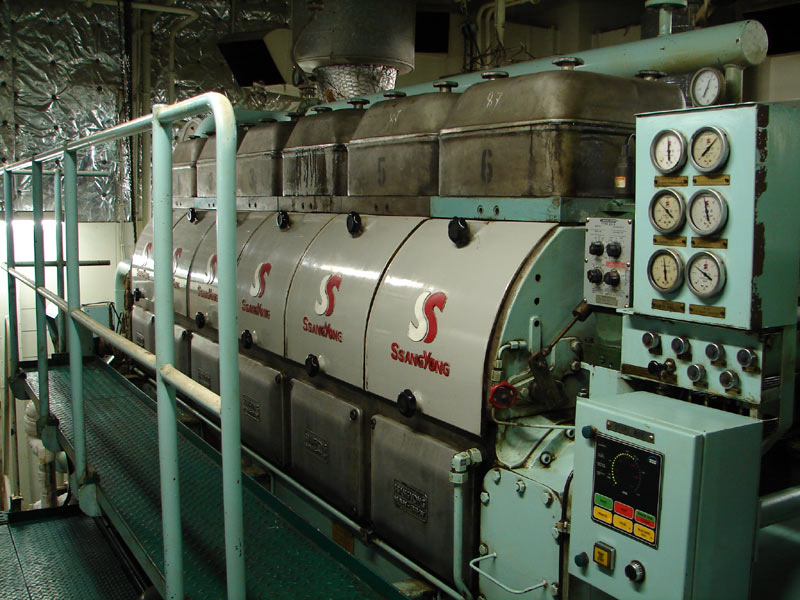
\includegraphics[width=0.49\textwidth]{images/photo_diesel_generateur.jpg}
			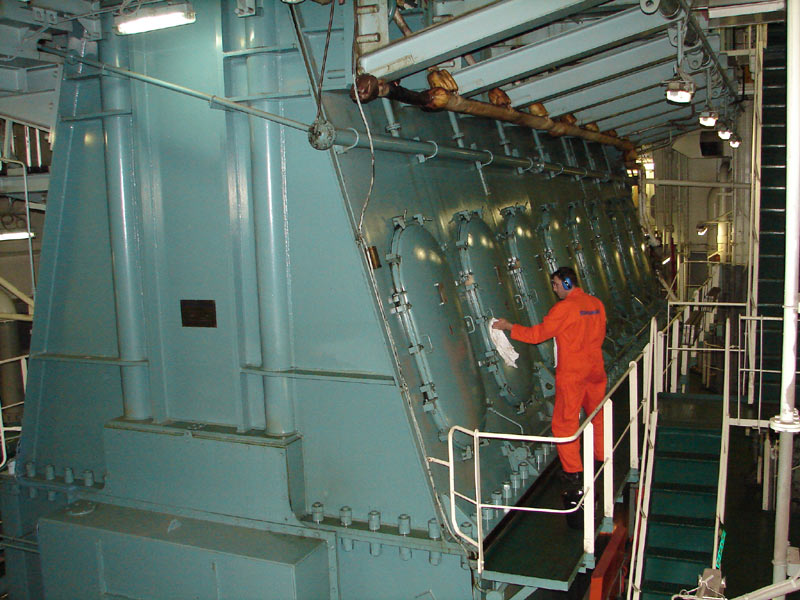
\includegraphics[width=0.49\textwidth]{images/photo_diesel_propulsion.jpg}
		\end{center}
		\supercaption{Moteurs Diesel six cylindres de~\SI{1100}{\kilo\watt} électrogène (gauche) et sept cylindres de~\SI{25}{\mega\watt} propulsif (droite) d’un pétrolier de~\SI{290 000}{\tonne}.}{\wcfile{Diesel generator on an oil tanker.jpg}{Photo 1} et \wcfile{Main engine of a VLCC tanker 3.jpg}{2} \ccbysa par Hervé Cozanet}
	\end{figure}

	\begin{itemize}
		\item La compression et la détente sont isentropiques :
		\item La combustion est à pression constante ;
		\item Le rejet de chaleur est à volume constant.
		\item Au début du cycle, l’air est à~\SI{15}{\degreeCelsius} et~\SI{1}{\bar} ;
		\item La chaleur spécifique fournie chaque cycle est de~\SI{400}{\kilo\joule\per\kilogram}. 
		\item Le taux de compression $\frac{V_\text{max.}}{V_\text{min.}}$ est de~\num{16}.
	\end{itemize}
	
	\begin{enumerate}
		\item Tracez le cycle thermodynamique suivi sur un diagramme pression-volume ou tem\-pérature-entropie, en indiquant tous les transferts de chaleur et de travail.
		\item Quelle est la température de l’air après la compression ?
		\item Quelle est la température de l’air après la combustion ?
		\item Montrez que lors de l’apport de chaleur, le rapport des volumes est égal au rapport des températures, et calculez ainsi la température à la fin de la détente.
		\item Quel est le rendement du moteur ?
		\item Il est aisé de montrer qu’à taux de compression égal, un cycle Diesel est moins efficace qu’un cycle dit «~à essence~» (cycle d’Otto). Pourquoi est-il alors utilisé ?
	\end{enumerate}

\exercisesolutionpage
\subsubsection*{Résultats}
	\linktosolutionsblurb
	
	\begin{description}
		\item [10.2] 
	 		\tab 2) $T_\text{entrée cc} = \SI{647,1}{\kelvin}$, $T_\text{échap} = \SI{738,1}{\kelvin}$, $w_\text{net} = \SI{-168,45}{\kilo\joule\per\kilogram}$ \\
	 		\tab 3) $\eta_\text{mot.} = \SI{26,49}{\percent}$ ; $r_{w} = \SI{31,71}{\percent}$ 
	 		\tab 5) $w_\text{comp.} = \SI{+333,7}{\kilo\joule\per\kilogram}$ :\\ $w_\text{net} = \SI{-187,6}{\kilo\joule\per\kilogram}$ 
	 		\tab 6) $\eta_\text{mot.} = \SI{25,28}{\percent}$ (\SI{-1,2}{pt}).
		\item [10.3] 
	 		\tab 2) $T_{B} = \SI{570,7}{\kelvin}$ 
	 		\tab 3) $T_{D} = \SI{880,9}{\kelvin}$ 
	 		\tab 4) $\dot{W}_\text{hélices} = \SI{1,025}{\mega\watt}$ 
	 		\tab 5) Une possibilité : augmenter $\dot{m}_\text{moteur}$ sans modifier les températures. Alors, $\dot{m}_\text{entrée~moteur~2} = \SI{5,096}{\kilogram\per\second}$.
		\item [10.4] 
	 		\tab 2) $T_{2} = \SI{785,2}{\kelvin}$, $T_{4is.} = \SI{783,6}{\kelvin}$ : $p_4 = \SI{3,13}{\bar}$ 
	 		\tab 3) $C_{5} = \SI{714,3}{\metre\per\second}$ (mais les tuyères ne sont jamais isentropiques…)
	 		\tab 4) $p_6 = \SI{4,684}{\bar}$ 
	 		\tab 5) $C_{7}= \SI{811,3}{\metre\per\second}$ (idem).
		\item [10.5] 
	 		\tab 2) $T_{2} = \SI{640,3}{\kelvin}$ et $T_{3} = \SI{1257,8}{\kelvin}$ 
	 		\tab 3) $q_{4\to 1} = \SI{-295,2}{\kilo\joule\per\kilogram}$
	 		\tab 4) $\eta_\text{moteur} = \SI{41}{\percent}$
	 	\item [10.6]
	 		\tab 2) $T_{2} = \SI{873,1}{\kelvin}$
	 		\tab 3) $T_{3} = \SI{1271,1}{\kelvin}$ 
	 		\tab 4) $T_{4} = \SI{572,2}{\kelvin}$
	 		\tab 5) $\eta_\text{moteur} = \SI{41,5}{\percent}$
	\end{description}

